In this chapter, the details of implementation will be discussed. It starts with an overview and the architecture of the blockchain enabled logistic application, and is followed by three important component in the application: transaction, the consensus, and the flow. In the next section, we provide a UML class diagram and several tables to describe the functionalities of the classes. However, all the structures and designs are based on the Corda platform. 

\section{Architecture}


\begin{outline}
	\1 Storage services and vaults backed by a SQL DB
	  \2 Default DB is h2  
	\1 RPC client framework and server shell for communication amongst network nodes
	\1 Customized functionality called CorDapps.
	   \2 States, Flows, Contracts are essential for CorDapps.
	\1 ServiceHub internal contains references to the 8 service features(in Figure 6.3, the 8 blocks beneath ServiceHub, except Storage Service)
\end{outline}

\begin{figure}[!htb]% order of placement preference: here, top, bottom
	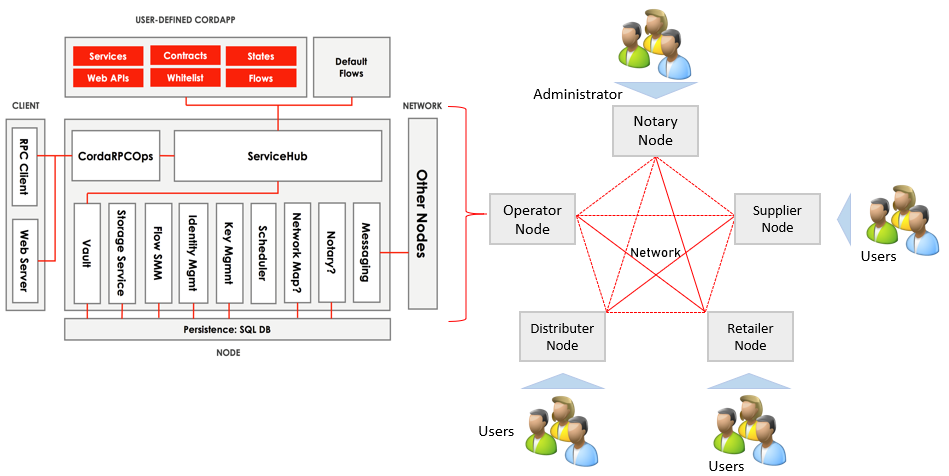
\includegraphics[width=\textwidth]{charts/node-architecture}
	\caption{The architecture of a single node}
\end{figure}

%=========================================================================
\section{Key Components}
This part provides in-depth information of about Corda's components, which helps audience better master the inner logic of the platform. It's critical for successful development.

\subsection{Roles in Corda}


\subsection{Corda Network}

	
\subsection{Corda Ledger}

\subsection{States}

\subsection{Contracts}

\subsection{Flows}

\subsection{Consensus}

%=========================================================================
\section{UML}
\subsection{Action Sequence}


Next Chapter we will demonstrate the performance and the correctness of our system.